\documentclass[10pt,graphics,aspectratio=169,table]{beamer}
\usepackage{listings}
\usepackage{amsmath}
\usepackage{hyperref}
\usepackage{listings}

\usetheme{metropolis}
\title{Suckless}
\subtitle{Software that sucks less}
\author{Jannusch Bigge}
\lstset{language=bash}
\titlegraphic{\hfill
\includegraphics[height=1.25cm]{../logo}}
\begin{document}
\begin{frame}[plain]
    \maketitle
\end{frame}

\begin{frame}{Outline}
    \tableofcontents
\end{frame}

\section{Philosophy}
\begin{frame}{Philosophy}
	\begin{quotation}
		"We are the home of quality software[...]"
		
		\begin{flushright}
			--- suckless.org
		\end{flushright}
	\end{quotation}
\end{frame}

\note{This is a note}

\begin{frame}{Philosophy}
	\framesubtitle{What makes suckless so special?}
	\begin{itemize}
		\item focus on simplicity, clarity and frugality
		\item keeping things simple, minimal and usable
		\item focuses on advanced and experienced computer users
	\end{itemize}
\end{frame}

\begin{frame}{Philosophy}{Why suckless software is better}
	Avoid bloated software
	\begin{itemize}
		\item Code complexity is the mother of bloated software
		\item vulnerabilities become commonplace
		\end{itemize}
\end{frame}

\section{Basics}

\begin{frame}{Basics}
	\begin{itemize}
		\item open source
		\item compile it yourself
		\item written in C
		\item divided into programs and tools
	\end{itemize}	
\end{frame}

\begin{frame}{Coding Style}
	 \begin{itemize}
	 	\item keep your style {\bf consistent}
	 	\item maintainer of the project define style
	 	\item some references: openbsd and pikestyle (Rob Pike)
	 \end{itemize}
\end{frame}

\section{Example projects}

\begin{frame}{Examples - Bad sh**}
	\begin{figure}
		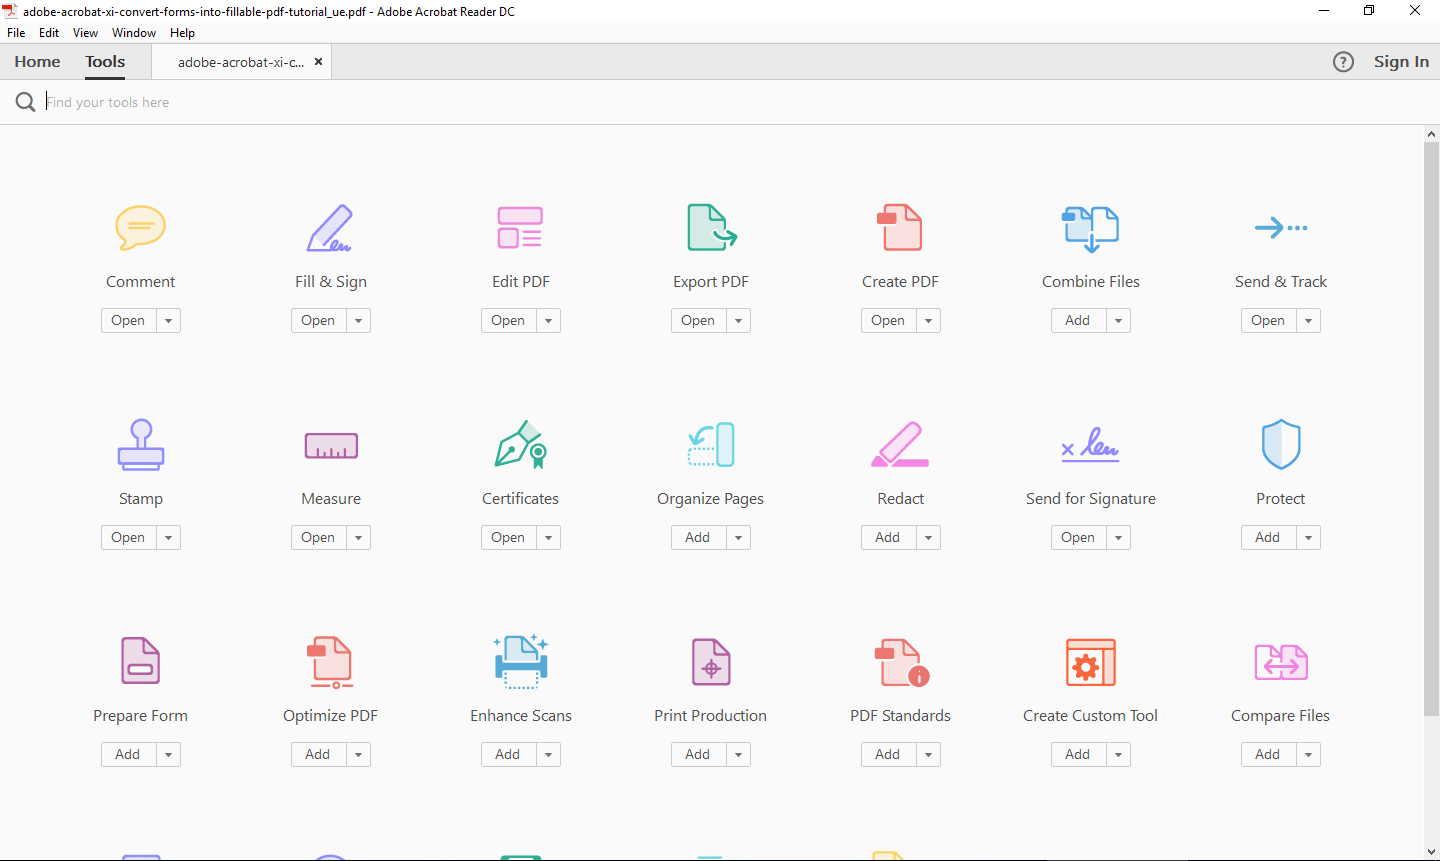
\includegraphics[scale=0.2]{Adobe-Acrobat-Reader-DC-Screen-1.png}
		\caption{https://windows10top.com/wp-content/uploads/2017/03/Adobe-Acrobat-Reader-DC-Screen-1.png}
	\end{figure}	
\end{frame}

\begin{frame}{Projects}{Some known projects}
	\begin{itemize}
		\item dmenu
		\item dwm
		\item st
		\item surf
	\end{itemize}
	
\end{frame}

\begin{frame}{Projects}
    \section*{dmenu}
    \subsection{dmenu}
\end{frame}

\begin{frame}{dmenu}{A menu for every situation}
	\begin{itemize}
		\item only a menu that lists things
		\item usable with own content
		\item usable in ci with other commands (grep, pipe...)
	\end{itemize}
\end{frame}

\begin{frame}{Projects}
    \section*{dwm - a tiling window manager}
    \subsection{dwm}
\end{frame}

\begin{frame}{dwm} 
	\begin{itemize}
		\item one prioritized window
		\item other windows organized in one specific pattern 
		\item other patterns possible
	\end{itemize}
\end{frame}

\begin{frame}{dwm}
    \begin{figure}
        \centering
        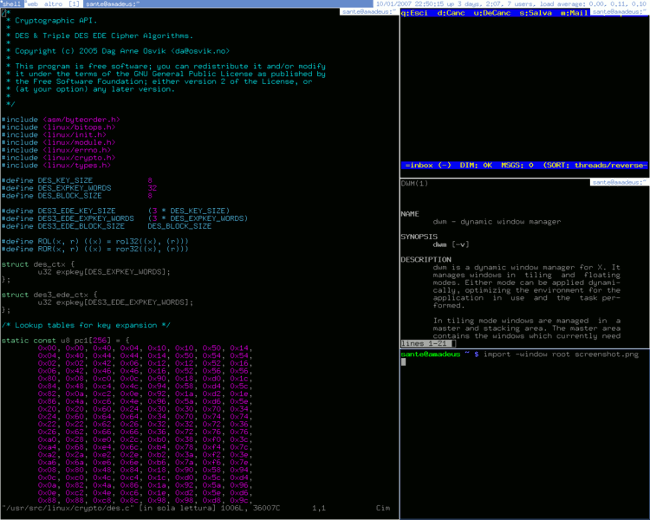
\includegraphics[scale=0.35]{DWM.png}
        \caption{http://linuxaria.com/wp-content/uploads/2013/04/DWM.png}
        \label{fig:my_label}
    \end{figure}
\end{frame}

\begin{frame}{Projects}
    \section*{st}
    \subsection{st}
\end{frame}

\begin{frame}{st - simple terminal}
Xterm is unmaintainable
\begin{itemize}
    \item xterm is bloated
    \item 65k lines of code
    \item emulates never needed terminals 
\end{itemize}
\end{frame}

\begin{frame}{st - simple terminal}
Implemented features of st
\begin{itemize}
    \item most VT10X escape sequences
    \item UTF-8
    \item 256 colors and true colors
    \item mouse and keyboard shortcuts (via config.h)
    \item and many more
\end{itemize}
\end{frame}

\begin{frame}{st - simple terminal}
st is still in active development
\begin{itemize}
    \item having a working terminal
    \item not reimplementing tmux and comrades
    \item \href{https://git.suckless.org/st/file/TODO.html}{TODOS}
\end{itemize}
\end{frame}

\begin{frame}{Projects}
\section*{surf}
\subsection{surf}
\end{frame}

\begin{frame}{surf}
Its a web browser - only a web browser
% XEmbed protocol support
\end{frame}

\begin{frame}{practice}
    \section*{And now something completely different}

\end{frame}
\begin{frame}{practice}
    \section{practice}
\end{frame}

\begin{frame}{practice}
What I will show you:
    \begin{itemize}
        \item install surf, tabbed and dmenu
        \item patch surf with search engine and bookmarks
        \item fix the patch ;)
        \item show how bookmarks work
        \item enjoy the final result
    \end{itemize}
\end{frame}

\begin{frame}[fragile]{Installation}
	program = surf, tabbed, dmenu
	\begin{lstlisting}
$git clone https://git.suckless.org/${program}
$cd ${program}
$sudo make install clean
$./${program}
\end{lstlisting}

\end{frame}

\begin{frame}{Patch}
	download the patch in the same file as surf
	
	\texttt{patch -p1 < surf-git-20170323-webkit2-searchengines.diff}
\end{frame}

\begin{frame}{Fix the patch}
	Don't ask why, but there is an error in the patch...
	\begin{figure}
		\includegraphics[scale=0.4]{Noice.jpg}
		\caption{https://memegenerator.net/img/instances/68375583/noice.jpg}
	\end{figure}
\end{frame}



\begin{frame}{Configuration}
	open \texttt{config.h} as \textbf{sudo} and configure what ever you want
\end{frame}
	

\end{document}
